\documentclass{beamer}
%
% Choose how your presentation looks.
%
% For more themes, color themes and font themes, see:
% http://deic.uab.es/~iblanes/beamer_gallery/index_by_theme.html
%
\mode<presentation>
{
  \usetheme{default}      % or try Darmstadt, Madrid, Warsaw, ...
  \usecolortheme{default} % or try albatross, beaver, crane, ...
  \usefonttheme{default}  % or try serif, structurebold, ...
  \setbeamertemplate{navigation symbols}{}
  \setbeamertemplate{caption}[numbered]
} 

\usepackage[english]{babel}
\usepackage[utf8x]{inputenc}

\title[Your Short Title]{Noise evaluation and reduction}
\author{Hoang Duc Viet}
\institute{ICT Lab}
\date{\today}

\begin{document}

\begin{frame}
  \titlepage
\end{frame}

% Uncomment these lines for an automatically generated outline.
%\begin{frame}{Outline}
%  \tableofcontents
%\end{frame}

\section{Introduction}

\begin{frame}{Introduction}

Denoising is considered as one of the major issues in image processing.
The noise in an image can be due to camera sensors, atmospheric conditions or transmission through a medium. Denoising has its root in wide range of applications such as segmentation, recognition, classification etc.
\vspace{1cm} 
\begin{itemize}
  \item Problem
  
  \
  
  \item Solution
  
  \
  
  \item Evaluation
  
  \
  
  \item Conclusion
\end{itemize}

%\vskip 1cm

%\begin{block}{Examples}
%Some examples of commonly used commands and features are included, to help you get started.
%\end{block}

\end{frame}

\section{Some \LaTeX{} Examples}

\subsection{Noise}

\begin{frame}{Problem}

%\textbf{Definition}

%\vspace{0.5cm}

\begin{itemize}



\item Noise:

Noise is the cause of errors from image when in pixel values that do not reflect the true intensities of the
real scene.

\vspace{7mm}

\item Denoise:

Noise removal is popular solution for photography or improve the image was degraded.


\end{itemize}




% Commands to include a figure:
%\begin{figure}
%\includegraphics[width=\textwidth]{your-figure's-file-name}
%\caption{\label{fig:your-figure}Caption goes here.}
%\end{figure}

%\begin{table}
%\centering
%\begin{tabular}{l|r}
%Item & Quantity \\\hline
%Widgets & 42 \\
%Gadgets & 13
%\end{tabular}
%\caption{\label{tab:widgets}An example table.}
%\end{table}

\end{frame}

\subsection{Type of noise}

\begin{frame}{Type of noise}
%\textbf{Definition}

%\vspace{0.5cm}

\begin{itemize}
	\item Fixed Pattern
	
%	Appear during extremely long exposures

	
	\
	
	\item  Random Noise
	
%	Maybe the most common image noise
	
	\
	
	\item Banding Noise
	
%	Dependent on what type of camera we are using
\end{itemize}

\end{frame}


\subsection{Fixed Pattern}
\begin{frame}{Fixed Pattern}
Fixed-pattern noise (FPN) is the term given to a particular noise pattern on digital imaging sensors. 
\vspace{1cm}
\begin{center}
	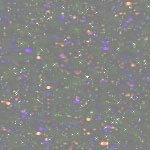
\includegraphics{fix.png}

Long Exposure

Low ISO Speed
\end{center}

\end{frame}

\subsection{Random Noise}
\begin{frame}{Random Noise}
Random noise is characterized by intensity and color fluctuations above and below the actual image intensity.
\vspace{1cm}
\begin{center}
	
\includegraphics{random.png}

Short Exposure

High ISO Speed
\end{center}
\end{frame}

\subsection{Banding Noise}
\begin{frame}{Banding Noise}
Banding noise is highly camera-dependent, and is noise which is introduced by the camera when it reads data from the digital sensor. 
\vspace{1cm}
\begin{center}
	
\includegraphics{banding.png}

Susceptible Camera

Brightened Shadows
\end{center}
\end{frame}
\subsection{Quality Of Camera}
\begin{frame}{Quality Of Camera}
Quality Of Camera is hard problem though our technology have more improvement. So the quality of the camera is evaluated when it solves the following 3 problems as below :
\vspace{1cm}
\begin{center}
	\begin{itemize}
		\item Increases with the light
		\item Sensor became heats up
		\item Long exposures
	\end{itemize}
\end{center}

\end{frame}
\subsection{Solution}

\begin{frame}{Solution}
%\textbf{Definition}

%\vspace{0.5cm}
\begin{itemize}
	\item Spatial Filtering
	
	 In spatial domain methods, the denoising procedure is directly applied on pixels.

	
	\
	
	\item  Filtering Method
	
They will help image restoration is to remove the noise from the image in such a way that the original image is the best quality
	
	
\end{itemize}

\end{frame}

\subsection{Type Of Filtering}

\begin{frame}{Type Of Filtering}
%\textbf{Definition}

%\vspace{0.5cm}
\begin{itemize}
	\item Median Filter
	
%	A nonlinear digital filtering technique
	
	
	\
	
	\item  Average Filter
	
%To replace each pixel value in an image with the mean(’average’)
	
	\
	
		\item Gaussian Filter
		
%		 have feature of having no overshoot to a step function input while minimizing the rise and fall time
	
	
	\
	
	\item  Wiener Filter
	
%	minimizes the mean square error between the estimated random process and the desired process
\end{itemize}

\end{frame}

\subsection{Median Filter}
\begin{frame}{Median Filter}

Median Filtering is very widely used in image processing and it preserves edges while removing noise. (speckle noise \& salt-pepper noise)




\vspace{2cm}

\begin{tabular}{|c|c|c|}  
	\hline 
	30 & 10 & 20 \\ 
	\hline                    
	10 & 250 & 25 \\ 
	\hline 
	20 & 25 & 30 \\ 
	\hline 
\end{tabular} 

\

\

$\Rightarrow$ 10 10 20 20 25 25 30 30 250 

\hspace{26mm}$\uparrow$

\hspace{20mm} median
\end{frame}

\subsection{Average Filter}
\begin{frame}{Average Filter}
Average filter is useful for removing grain noise from a photograph.
%Because each pixel gets set to the average of the pixels in its neighborhood, local variations caused by grain are reduced. 


\vspace{1cm}
\begin{center}

	Filter 3$\times$3
	
	$\dfrac{1}{9}\begin{tabular}{|c|c|c|}
	\hline 
	1 & 1 & 1 \\ 
	\hline 
	1 & 1 & 1 \\ 
	\hline 
	1 & 1 & 1 \\ 
	\hline 
	\end{tabular}$ 	
\end{center}

\begin{center}
	Filter 5$\times$5
	
	$\dfrac{1}{25}\begin{tabular}{|c|c|c|c|c|}
	\hline 
	1 & 1 & 1 & 1 & 1 \\ 
	\hline 
	1 & 1 & 1 & 1 & 1 \\ 
	\hline 
	1 & 1 & 1 & 1 & 1 \\ 
	\hline 
	1 & 1 & 1 & 1 & 1 \\ 
	\hline 
	1 & 1 & 1 & 1 & 1 \\ 
	\hline 
	\end{tabular} $
\end{center}



\end{frame}

\subsection{Average Filter(1)}
\begin{frame}{Average Filter(1)}
\begin{center}
	Filter 7$\times$7
	
	$\dfrac{1}{49}\begin{tabular}{|c|c|c|c|c|c|c|}
	\hline 
	1 & 1 & 1 & 1 & 1 & 1 & 1 \\ 
	\hline 
	1 & 1 & 1 & 1 & 1 & 1 & 1 \\ 
	\hline 
	1 & 1 & 1 & 1 & 1 & 1 & 1 \\ 
	\hline 
	1 & 1 & 1 & 1 & 1 & 1 & 1 \\ 
	\hline 
	1 & 1 & 1 & 1 & 1 & 1 & 1 \\ 
	\hline 
	1 & 1 & 1 & 1 & 1 & 1 & 1 \\ 
	\hline 
	1 & 1 & 1 & 1 & 1 & 1 & 1 \\ 
	\hline 
	\end{tabular} $
\end{center}
\end{frame}

\subsection{Gaussian Filter}
\begin{frame}{Gaussian Filter}

Gaussian filtering is used to blur images and remove noise and detail.
\vspace{0.5cm}

The Gaussian kernel in dimension 2:


$G(x,y) = \dfrac{1}{2\pi\sigma^2}\exp\left[-\dfrac{(x-\mu_x)^2+(y-\mu_y)^2}{2\sigma^2}\right ]$

\hspace{3cm}$$\Updownarrow$$

\hspace{3cm}$G(x,y)=\dfrac{1}{2\pi\sigma^2}e^{-{\dfrac{x^2+y^2}{2\sigma^2}}}$	

\vspace{0.5cm}

Define the Gaussian mask($\sigma$=1):
%$$\mu = 0$$
%$$\sigma = 0.8$$
\begin{center}
	Filter 3$\times$3
	
	$\dfrac{1}{16}\begin{tabular}{|c|c|c|}
	\hline 
	1 & 2 & 1 \\ 
	\hline 
	2 & 4 & 2 \\ 
	\hline 
	1 & 2 & 1 \\ 
	\hline 
	\end{tabular} $
\end{center}
\end{frame}

\subsection{Gaussian Filter(1)}
\begin{frame}{Gaussian Filter(1)}
\begin{center}
	Filter 5$\times$5
	
	$\dfrac{1}{273}\begin{tabular}{|c|c|c|c|c|}
	\hline 
	1 & 4 & 7 & 4 & 1 \\ 
	\hline 
	4 & 16 & 26 & 16 & 4 \\ 
	\hline 
	7 & 26 & 41 & 26 & 7 \\ 
	\hline 
	4 & 16 & 26 & 16 & 4 \\ 
	\hline 
	1 & 4 & 7 & 4 & 1 \\ 
	\hline 
	\end{tabular}$ 
\end{center}

\begin{center}
	Filter 7$\times$7
	
	$\dfrac{1}{1003}$\begin{tabular}{|c|c|c|c|c|c|c|}
		\hline 
		0 & 0 & 1 & 2 & 1 & 0 & 0 \\ 
		\hline 
		0 & 3 & 13 & 22 & 13 & 3 & 0 \\ 
		\hline 
		1 & 13 & 59 & 97 & 59 & 13 & 1 \\ 
		\hline 
		2 & 22 & 97 & 159 & 97 & 22 & 2 \\ 
		\hline 
		1 & 13 & 59 & 97 & 59 & 13 & 1 \\ 
		\hline 
		0 & 3 & 13 & 22 & 13 & 3 & 0 \\ 
		\hline 
		0 & 0 & 1 & 2 & 1 & 0 & 0 \\ 
		\hline 
	\end{tabular} 
\end{center}
\end{frame}

\subsection{Wiener Filter}
\begin{frame}{Wiener Filter}

The Wiener filter is to filter out noise that has corrupted a signal.
\vspace{1cm}

Weiner filter are characterized by following:
\begin{itemize}
	\item Assumption :
	
	Stationary linear with known spectral characteristics or
	known autocorrelation and cross-correlation.


\

	\item Requirement:
	
	The filter must be physically realizable

\

	\item Performance criterion: 
	
	Minimum mean square error.

\end{itemize} 
\end{frame}

\subsection{Evaluation}
\begin{frame}{Evaluation}
The MSE is a measure of the quality of an estimator—it is always non-negative, and values closer to zero are better.


\

\begin{center}

	$MSE =  \dfrac{1}{n} \displaystyle \sum_{i=1}^{n}(\hat{Y_i} - Y_i)^2$
	

\end{center}
 

\end{frame}


\subsection{Evaluation}
\begin{frame}{Evaluation(1)}
\begin{center}
	
\begin{tabular}{|c|c|}

	\hline 
	Filter & MSE \\ 
	\hline 
	Median & 0.0372 \\ 
	\hline 
	Average & 0.0274 \\ 
	\hline 
	Gaussian & 0.0041 \\ 
	\hline 
	Weiner & 0.0372 \\ 
	\hline 
	SURE-LET & 3.22 \\ 
	\hline 
\end{tabular} 

\

Comparison Table
\end{center}
\end{frame}

\subsection{Conclusion}
\begin{frame}{Conclusion}
\begin{center}
\begin{itemize}
	\item The best of results
	
	 Gaussian filter with  MSE is minimum mean square error.

	
	\
    
    \item Future development
     
      Improvement of the proposed method over the existing approaches in terms of visual
     quality
\end{itemize}
\end{center}
 

\end{frame}



\subsection{}
\begin{frame}{}

\begin{center}
	\begin{LARGE}
		THANK YOU !!!
	\end{LARGE} 
\end{center}
\end{frame}








\end{document}
